% PointWorld presenter deck. CS 2883R, Wed 18 Nov 2026. Juntang Wang and Vivian Hui.
% Numbers checked against arXiv 2601.03782v1; each frame comment names its source.
% Rules: one claim per frame, at most 3 bullets, no bullet restating its own figure;
% teal marks PointWorld or the one number to carry; l2 errors are in metres, so 0.001 is
% 1 mm; zero-shot means no demos and no finetuning, not no human input (masks and targets
% are drawn by hand); equations, full tables and protocol details live in the backup.
% The presenter speaks as the first author (course guidelines): our critique lives in the
% Discussion questions and the "Our reading" backup, for the reviewer and red-team roles.
% 15:00 for two speakers, about 13:45 budgeted. Vivian S1-3 (to planning), Juntang S4-6.
% If long, cut "Why gripper points" first. LAPA deck: git tag lapa-final.
% Build: latexmk -pdf main.tex
\documentclass[aspectratio=169,12pt]{beamer}
\usetheme[progressbar=none, numbering=counter]{moloch}
%howdy
\usepackage[sfdefault,light]{FiraSans}
\usepackage[T1]{fontenc}
\usepackage{tikz}
\usepackage{booktabs}
\usepackage{multicol}
\usepackage[authoryear, round]{natbib}
\definecolor{cite}{HTML}{1F5FBF}  % citations and URLs: blue, clickable
\hypersetup{colorlinks=true, citecolor=cite, urlcolor=cite, linkcolor=.}
\renewcommand{\bibsection}{}                          % the frame title is enough
\bibliographystyle{plainnat}
% Beamer 3.77 + current hyperref leave natbib's \hyper@natlinkbreak empty, which drops the
% ", " in (Author et al., 2024) and the " (" in Author et al. (2024). Restore hyperref's definition.
\makeatletter
\AddToHook{begindocument/end}{%
  \def\hyper@natlinkbreak#1#2{\hyper@linkend#1\hyper@linkstart{cite}{cite.#2}}}
\makeatother

\definecolor{ink}{HTML}{222222}
\definecolor{mute}{HTML}{8a8a8a}
\definecolor{pw}{HTML}{12807A}       % PointWorld rows and accents
\definecolor{crimson}{HTML}{A51C30}  % Harvard; title slide only

\setbeamercolor{normal text}{fg=ink, bg=white}
\setbeamercolor{frametitle}{fg=ink, bg=white}
\setbeamercolor{page number in head/foot}{fg=mute}
\setbeamertemplate{itemize items}{\color{pw}--}
\setlength{\leftmargini}{1.1em}

\newcommand{\src}[1]{{\scriptsize\color{mute}\citep{#1}}}
\newcommand{\paperfig}[3]{%
  \begin{tikzpicture}[baseline=(f.south)]
    \node[inner sep=0pt] (f) {\includegraphics[#1]{#2}};
    \node[anchor=north east, inner sep=1pt, font=\tiny, text=mute] at (f.south east)
      {\citet{huang2026pointworld}, #3};
  \end{tikzpicture}}
\newcommand{\credit}[1]{\par\hfill{\tiny\color{mute}\citet{huang2026pointworld}, #1}\par}
\newcommand{\pw}[1]{{\color{pw}#1}}
\newcommand{\colhead}[2]{\begin{minipage}[t][1.5cm]{\linewidth}\raggedright
  {\small\bfseries #1}\\\src{#2}\end{minipage}\\}
\newenvironment{notes}[1][\linewidth]
  {\begin{minipage}{#1}\footnotesize\begin{itemize}\setlength{\itemsep}{2pt}}
  {\end{itemize}\end{minipage}}

\begin{document}

% 0. Title  0:15
\begin{frame}[plain]
  \vfill
  {\LARGE\bfseries PointWorld: Scaling 3D World Models\\[2pt]
    for In-The-Wild Robotic Manipulation}\\[6pt]

  {\scriptsize\color{mute} Wenlong Huang, Yu-Wei Chao, Arsalan Mousavian, Ming-Yu Liu,
    Dieter Fox, Kaichun Mo, Li Fei-Fei.\\ Stanford, NVIDIA.\
    CVPR 2026. arXiv 2601.03782. Code, data and checkpoints: github.com/NVlabs/PointWorld}

      \textcolor{crimson}{\rule{\textwidth}{0.8pt}}\\[8pt]
  Juntang Wang $\cdot$ Vivian Hui\\[2pt]
  \vfill
\end{frame}



% Abstract definition: orient the audience immediately after the title.
\begin{frame}{What is PointWorld?}
  \vfill
  \centering
  \begin{minipage}{0.92\textwidth}
    \large\raggedright
    ``POINTWORLD, a \textbf{large pre-trained 3D world model} that
    unifies \textbf{state and action} in a \textbf{shared 3D space}
    as \textbf{3D point flows}: given one or few RGB-D images and
    a sequence of low-level robot action commands, POINTWORLD
    forecasts \textbf{per-pixel displacements in 3D} that respond
    to the given actions.''
  \end{minipage}
  \vfill
  \credit{Abstract; emphasis added}
\end{frame}

%% ---- Part A (Vivian): expanded introduction, method, and planning ----
% Sources: PointWorld arXiv:2601.03782v1, Sections 1--3 and 5.2.
% Beamer overlays reveal content on successive clicks. Original theme is unchanged.
\newcommand{\lossmark}[3]{\ifnum#1=#2\relax{\color{orange!90!red}\setlength{\fboxrule}{2pt}\setlength{\fboxsep}{2.5pt}\boxed{\color{ink}#3}}\else#3\fi}
\newcommand{\pwequation}[1]{%
\[
\mathcal L=\tfrac12\sum_{k,i}^{H,N_S}
\lossmark{#1}{2}{w_{k,i}}
\Big(
\lossmark{#1}{1}{\rho_\delta(\hat{\mathbf P}_{t+k,i}-\mathbf P_{t+k,i})}
\lossmark{#1}{3}{e^{-s_{k,i}}}
+\lossmark{#1}{4}{s_{k,i}}
\Big).
\]}
% Introduction 1/3
\begin{frame}{Context: why do robots need world models?}
  \centering
  \paperfig{height=3.55cm}{figs/fig1_teaser.pdf}{Fig.~1}
  \vfill
  \begin{notes}[0.92\linewidth]
    \item<1-> A robot must anticipate how an action changes its surroundings before committing to it.
    \item<2-> A \textbf{world model} predicts future scene states from the current observation and a proposed action.
    \item<3-> \pw{Use these predictions to compare actions and plan physical interactions in unseen environments.}
  \end{notes}
  \vfill
\end{frame}

\newcommand{\approachcrop}[6]{%
  \begin{tikzpicture}
    \node[anchor=south west,inner sep=0pt] (ref) at (0,0)
      {\phantom{\includegraphics[width=#1]{#2}}};
    \begin{scope}[x={(ref.south east)},y={(ref.north west)}]
      \clip (#3,#4) rectangle (#5,#6);
      \node[anchor=south west,inner sep=0pt] at (0,0)
        {\includegraphics[width=#1]{#2}};
    \end{scope}
    \pgfresetboundingbox
    \begin{scope}[x={(ref.south east)},y={(ref.north west)}]
      \path[use as bounding box] (#3,#4) rectangle (#5,#6);
    \end{scope}
  \end{tikzpicture}%
}

\begin{frame}[t]{Related work: approaches to predicting physical interactions}
\vspace{-0.9cm}

\begin{columns}[t]

% ----- Physics simulators -----
\column{0.31\textwidth}
\uncover<1->{
  \begin{minipage}[t][0.8cm]{\linewidth}
    {\small\bfseries Physics simulators}\par
  \end{minipage}\par

  \begin{minipage}[c][1.95cm][c]{\linewidth}
    \centering
    \resizebox{!}{1.9cm}{%
      \approachcrop{8cm}{approach_mujoco.png}
        {0.30}{0.16}{0.72}{0.85}}
  \end{minipage}\par

  {\tiny\color{mute}
    \href{https://mujoco.readthedocs.io/en/stable/models.html}
      {MuJoCo Menagerie: Franka Panda}}\par

  \vspace{2pt}
  {\scriptsize
    \begin{itemize}
      \setlength{\itemsep}{3pt}
      \setlength{\parskip}{0pt}
      \setlength{\topsep}{2pt}
      \item Simulate physical interactions using equations,
        scene geometry, and specified physical properties.
      \item Require scene-specific setup, and simulated
        behavior can differ from reality.
    \end{itemize}
  }
}

% ----- Video generative models -----
\column{0.31\textwidth}
\uncover<2->{
  \begin{minipage}[t][0.8cm]{\linewidth}
    {\small\bfseries Video generative models}\par
  \end{minipage}\par

  \begin{minipage}[c][1.95cm][c]{\linewidth}
    \centering
    \resizebox{!}{1.9cm}{%
      \approachcrop{8cm}{approach_cosmos.jpg}
        {0.56}{0.25}{0.94}{0.82}}
  \end{minipage}\par

  {\tiny\color{mute}
    \href{https://www.nvidia.com/en-us/ai/cosmos/}
      {NVIDIA Cosmos: video generation}}\par

  \vspace{2pt}
  {\scriptsize
    \begin{itemize}
      \setlength{\itemsep}{3pt}
      \setlength{\parskip}{0pt}
      \setlength{\topsep}{2pt}
      \item Learn from video data to generate videos
        conditioned on inputs such as text or images.
      \item Realistic appearance does not guarantee accurate
        physics or precise robot-action control.
    \end{itemize}
  }
}

% ----- Learned dynamics models -----
\column{0.31\textwidth}
\uncover<3->{
  \begin{minipage}[t][0.8cm]{\linewidth}
    {\small\bfseries Learned dynamics\\models}\par
  \end{minipage}\par

  \begin{minipage}[c][1.95cm][c]{\linewidth}
    \centering
    \resizebox{!}{1.9cm}{%
      \approachcrop{8cm}{approach_dreamer.png}
        {0}{0.15}{0.51}{1}}
  \end{minipage}\par

  {\tiny\color{mute}
    \href{https://github.com/danijar/dreamerv3}
      {DreamerV3 (Hafner et al., 2025)}}\par

  \vspace{2pt}
  {\scriptsize
    \begin{itemize}
      \setlength{\itemsep}{3pt}
      \setlength{\parskip}{0pt}
      \setlength{\topsep}{2pt}
      \item Learn from interaction data to predict how
        the environment changes in response to actions.
      \item \textbf{Example: Dreamer} encodes a game screen
        into a latent state, then predicts how it changes
        after an action such as ``move right.''
    \end{itemize}
  }
}

\end{columns}
\vfill
\end{frame}

% Crops from the same example in Figure 2.
\newcommand{\pwvisualcrop}[5]{%
  \begin{tikzpicture}
    \node[anchor=south west,inner sep=0pt] (ref) at (0,0)
      {\phantom{\includegraphics[width=#1]{figs/fig2_overview.pdf}}};

    \begin{scope}[x={(ref.south east)},y={(ref.north west)}]
      \clip (#2,#3) rectangle (#4,#5);
      \node[anchor=south west,inner sep=0pt] at (0,0)
        {\includegraphics[width=#1]{figs/fig2_overview.pdf}};
    \end{scope}

    \pgfresetboundingbox
    \begin{scope}[x={(ref.south east)},y={(ref.north west)}]
      \path[use as bounding box]
        (#2,#3) rectangle (#4,#5);
    \end{scope}
  \end{tikzpicture}%
}

% Motivation for the representation, before introducing the core idea.
\begin{frame}[t]{Motivation: why use 3D point flows?}
  \vspace{-0.2cm}
  \footnotesize
  \begin{itemize}\setlength{\itemsep}{12pt}
    \item<1-> \textbf{\color{pw}Geometry for physical interaction}\\
      3D positions directly describe distances and contact geometry,
      rather than visual appearance alone.

    \item<2-> \textbf{\color{pw}A common format across robots}\\
      Point trajectories can describe different gripper shapes and
      robot embodiments without a fixed, robot-specific action vector.

    \item<3-> \textbf{\color{pw}Direct motion supervision}\\
      Corresponding scene points provide displacement targets.

    \item<4-> \textbf{\color{pw}Fewer required annotations}\\
      No explicit object segmentation or material labels are required
      as model inputs.
  \end{itemize}
  \vfill
  \credit{\S1--3.1}
\end{frame}

\begin{frame}[t]{PointWorld: state and action share 3D space}
\vspace{-0.35cm}
\centering

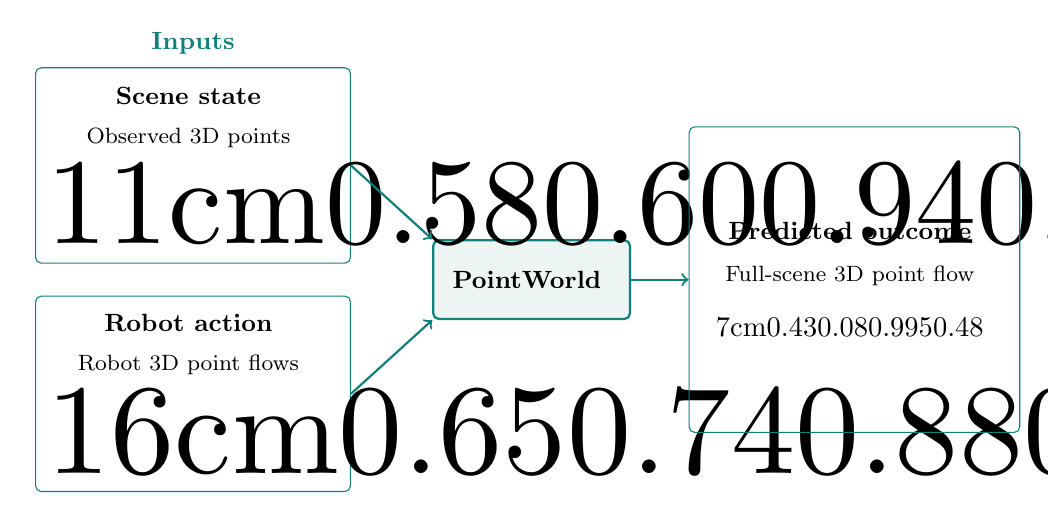
\begin{tikzpicture}[
  panel/.style={
    draw=pw,
    rounded corners=2pt,
    inner sep=4pt,
    align=center
  },
  model/.style={
    draw=pw,
    thick,
    fill=pw!8,
    rounded corners=2pt,
    minimum height=1cm,
    inner sep=7pt,
    align=center
  }
]

% Fixed bounds prevent movement between reveals.
\path[use as bounding box]
  (-2.1,-2.8) rectangle (10.5,3.2);

\node[font=\small\bfseries,text=pw]
  at (0,3.0) {Inputs};

% PointWorld model.
\node[model] (pwmodel) at (4.3,0) {
  \mbox{\small\bfseries PointWorld}
};

% Input 1: observed scene state.
\uncover<1->{
  \node[panel] (scene) at (0,1.45) {
    \begin{minipage}[c][2.2cm][c]{3.6cm}
      \centering

      {\small\bfseries Scene state}\par
      \vspace{2pt}

      {\footnotesize Observed 3D points}\par
      \vspace{5pt}

      \resizebox{!}{1cm}{%
        \pwvisualcrop{11cm}{0.58}{0.60}{0.94}{0.76}}
    \end{minipage}
  };

  \draw[->,thick,pw]
    (scene.east) -- (pwmodel.north west);
}

% Input 2: proposed robot action.
\uncover<2->{
  \node[panel] (action) at (0,-1.45) {
    \begin{minipage}[c][2.2cm][c]{3.6cm}
      \centering

      {\small\bfseries Robot action}\par
      \vspace{2pt}

      {\footnotesize Robot 3D point flows}\par
      \vspace{5pt}

      \resizebox{!}{1.05cm}{%
        \pwvisualcrop{16cm}{0.65}{0.74}{0.88}{0.94}}
    \end{minipage}
  };

  \draw[->,thick,pw]
    (action.east) -- (pwmodel.south west);
}

% Output: predicted scene motion.
\uncover<3->{
  \node[panel] (outcome) at (8.4,0) {
    \begin{minipage}[c][3.6cm][c]{3.8cm}
      \centering

      {\small\bfseries Predicted outcome}\par
      \vspace{3pt}

      {\footnotesize Full-scene 3D point flow}\par
      \vspace{8pt}

      \resizebox{3.4cm}{!}{%
        \pwvisualcrop{7cm}{0.43}{0.08}{0.995}{0.48}}
    \end{minipage}
  };

  \draw[->,thick,pw]
    (pwmodel.east) -- (outcome.west);
}

\end{tikzpicture}

\credit{Fig.~2, cropped; \S3.1}
\end{frame}

\begin{frame}{Contributions}
  \vfill
  \begin{itemize}\setlength{\itemsep}{16pt}
    \item<1-> A large pretrained \pw{3D world model} with a shared point-flow representation of scene state and robot action.
    \item<2-> A curated, open-source 3D interaction dataset: approximately \pw{2M trajectories and 500 hours} of real and simulated interaction.
    \item<3-> A \pw{single pretrained checkpoint} supports diverse real-robot manipulation tasks from one RGB-D capture, without extra demonstrations or post-training.
  \end{itemize}
  \vfill
  \credit{\S1, contributions}
\end{frame}




% Architecture walkthrough: coordinates normalized to Figure 2.
\newcommand{\pwarchrect}[4]{%
  \draw[orange!90!red,line width=2.8pt,rounded corners=2pt,
    preaction={draw=white,line width=5pt}]
    (#1,#2) rectangle (#3,#4);}
\newcommand{\pwarchitecturefocus}[2]{%
  \begin{tikzpicture}
    \node[anchor=south west,inner sep=0pt] (arch) at (0,0)
      {\includegraphics[height=#1]{figs/fig2_overview.pdf}};
    \begin{scope}[x={(arch.south east)},y={(arch.north west)}]
      \ifcase#2\relax
      \or % 1: RGB-D observation.
        \pwarchrect{0.004}{0.505}{0.414}{0.846}
      \or % 2: Full robot-action input.
        \pwarchrect{0.002}{0.851}{0.421}{0.997}
        \pwarchrect{0.002}{0.251}{0.220}{0.489}
      \or % 3: PTv3 backbone.
        \pwarchrect{0.224}{0.012}{0.414}{0.488}
      \or % 4: Concatenated point cloud.
        \pwarchrect{0.427}{0.502}{0.998}{0.978}
      \or % 5: Predicted full-scene point flow.
        \pwarchrect{0.427}{0.014}{0.998}{0.489}
      \or % 6: Scene points and DINOv3.
        \pwarchrect{0.002}{0.012}{0.219}{0.245}
      \or % 7: URDF and joint-action conversion.
        \pwarchrect{0.002}{0.851}{0.421}{0.997}
      \or % 8: Robot flows and time embedding.
        \pwarchrect{0.002}{0.251}{0.220}{0.489}
      \fi
    \end{scope}
    \pgfresetboundingbox
    \path[use as bounding box]
      (arch.south west) rectangle (arch.north east);
  \end{tikzpicture}%
}

\begin{frame}{Architecture overview}
  \centering
  \paperfig{height=5.7cm}{figs/fig2_overview.pdf}{Fig.~2}
\end{frame}


\begin{frame}{Architecture: scene state}
  \centering

  \begin{tikzpicture}
    \node[anchor=south west,inner sep=0pt] (arch) at (0,0)
      {\includegraphics[height=5.7cm]{figs/fig2_overview.pdf}};

    \begin{scope}[x={(arch.south east)},y={(arch.north west)}]
      % Highlight RGB-D observation
      \pwarchrect{0.004}{0.505}{0.414}{0.846}

      % Highlight scene points + DINOv3 features
      \pwarchrect{0.002}{0.012}{0.219}{0.245}
    \end{scope}
  \end{tikzpicture}

  \credit{Fig.~2, highlighted; \S3.1}
\end{frame}

\begin{frame}[t]{Scene state representation: 3D points and visual features}
\vspace{-0.3cm}

{\centering\small
  $\displaystyle
    \mathbf s_t
    =\{(\mathbf p_{t,i},\mathbf f_i^S)\}_{i=1}^{N_S}
  $\par
}

\vspace{0.7cm}
\begin{columns}[t]
  \column{0.48\textwidth}
  \uncover<1->{
    {\small\bfseries\color{pw}3D positions:
      $\mathbf p_{t,i}\in\mathbb R^3$}\par
    \vspace{6pt}
    \footnotesize
    \begin{itemize}\setlength{\itemsep}{9pt}
      \item Back-project calibrated RGB-D into a 3D scene point cloud.
      \item $\mathbf p_{t,i}$ is point $i$'s position at time $t$;
        $N_S$ is the number of observed scene points.
    \end{itemize}
  }

  \column{0.48\textwidth}
  \uncover<2->{
    {\small\bfseries\color{pw}Visual features:
      $\mathbf f_i^S\in\mathbb R^{D_S}$}\par
    \vspace{6pt}
    \footnotesize
    \begin{itemize}\setlength{\itemsep}{9pt}
      \item Attach features from a \textbf{frozen DINOv3 encoder}
        at corresponding image locations.
      \item These features provide appearance and objectness cues.
      \item The feature vector stays fixed during the imagined rollout.
    \end{itemize}
  }
\end{columns}
\vfill
\credit{\S3.1; \S5.1, pretrained 2D features}
\end{frame}


\begin{frame}{Architecture: robot action}
  \centering

  \begin{tikzpicture}
    \node[anchor=south west,inner sep=0pt] (arch) at (0,0)
      {\includegraphics[height=5.7cm]{figs/fig2_overview.pdf}};

    \begin{scope}[x={(arch.south east)},y={(arch.north west)}]
      % Top: URDF and proposed robot joint trajectory
      \pwarchrect{0.002}{0.851}{0.421}{0.997}

      % Bottom: robot point flows and time embeddings
      \pwarchrect{0.002}{0.251}{0.220}{0.489}
    \end{scope}
  \end{tikzpicture}

  \credit{Fig.~2, highlighted; \S3.1}
\end{frame}




\begin{frame}{Robot action representation: joints to 3D points}
  \vspace{-5pt}
  \[
    \mathbf r_{t+k,j}
    =
    \operatorname{FK}_{\mathrm{URDF}}
    (\mathbf q_{t+k},\mathbf u_j)
  \]

  \begin{columns}[T,onlytextwidth]
    \column{0.49\textwidth}
    {\small\bfseries\color{pw}Given robot geometry and motion}\par
    \vspace{6pt}
    \footnotesize
    \begin{itemize}\setlength{\itemsep}{9pt}
      \item<1-> \textbf{URDF}: robot links, joints, and geometry.
      \item<2-> $\mathbf u_j$: a sampled surface point fixed to a robot link.
      \item<3-> $\mathbf q_{t+k}$: proposed joint configuration at future step $k$.
    \end{itemize}

    \column{0.47\textwidth}
    {\small\bfseries\color{pw}Construct the point-flow action}\par
    \vspace{6pt}
    \footnotesize
    \begin{itemize}\setlength{\itemsep}{10pt}
      \item<4-> Forward kinematics computes each point's future 3D position,
        $\mathbf r_{t+k,j}$.
      \item<4-> Repeat over the proposed trajectory.
        In practice, sample \pw{300--500 points per gripper}.
    \end{itemize}
  \end{columns}
  \vfill
  \credit{\S3.1, action representation; \S5.2}
\end{frame}


% ----- Architecture and prediction in one slide -----
\begin{frame}{Architecture: predicting 3D displacement}
  \begin{columns}[c]

    \column{0.48\textwidth}
      \centering
      % Highlight follows the explanation.
      \only<1>{\pwarchitecturefocus{5.0cm}{4}}
      \only<2>{\pwarchitecturefocus{5.0cm}{3}}
      \only<3->{\pwarchitecturefocus{5.0cm}{5}}

    \column{0.48\textwidth}
      \footnotesize
      \begin{itemize}\setlength{\itemsep}{10pt}

        \item<1-> \textbf{Combine inputs}:
          concatenate scene points and proposed robot
          point trajectories into one point cloud.

        \item<2-> \textbf{PTv3 backbone}:
          process the combined cloud to produce
          learned features for each point.

        \item<3-> \textbf{MLP prediction head}:
          convert scene-point features into
          3D displacements.

      \end{itemize}

    
  \end{columns}
  \credit{Fig.~2, highlighted; \S3.1;
    PTv3 \citep{wu2023ptv3}}
\end{frame}


% ----- A distinct question: how far ahead? -----
\begin{frame}[t]{Prediction horizon = 10 futures states at once}
\vspace{-0.25cm}
\small

\textbf{Single-step prediction}
\[
  \hat{\mathbf s}_{t+1}
  =
  \mathcal F_\theta(\mathbf s_t,\mathbf a_t)
\]
{\footnotesize
  Predict one future state, then repeat to look further ahead.
\par}

\vspace{10pt}

\uncover<2->{
  \textbf{\pw{PointWorld: chunked prediction}}
  \[
    \mathcal F_\theta^H
    \big(\mathbf s_t,\mathbf a_{t:t+H-1}\big)
    =
    \hat{\mathbf s}_{t+1:t+H}
  \]
  {\footnotesize
    Predict $H=10$ future states in one forward pass:
    $0.1\,\mathrm{s}$ per step, covering $1\,\mathrm{s}$.
  \par}
}

\vspace{10pt}

\uncover<3->{
  {\footnotesize\bfseries Advantages}\par
  \begin{itemize}\setlength{\itemsep}{6pt}
    \item \footnotesize Better temporal consistency
      and less rollout drift.
    \item \footnotesize One forward pass per chunk,
      rather than repeated single-step predictions.
  \end{itemize}
}

\vfill
\credit{\S3.1; chunking ablation in \S5.2, Fig.~12}
\end{frame}


% Four successive overlays keep the equation fixed and move the highlight.
\begin{frame}{Training objective: Huber residual}
  \small
  \pwequation{1}
  \vspace{7pt}

  \begin{itemize}
    \footnotesize
    \setlength{\itemsep}{9pt}

    \item<1-> $\hat{\mathbf P}_{t+k,i}$ and $\mathbf P_{t+k,i}$: predicted and ground-truth future positions.

    \item<2-> Position error equals displacement error since the initial point is shared.

    \item<3-> $\rho_\delta$ is the elementwise \textbf{Huber loss}: quadratic for small residuals and linear for large ones, reducing sensitivity to noisy labels.

  \end{itemize}

  \vfill
  {\scriptsize\color{mute}
    Sum over future steps $k=1,\ldots,H$ and scene points $i=1,\ldots,N_S$.
  \par}
  \credit{Eq.~1, \S3.1}
\end{frame}


\begin{frame}{Training objective: emphasize moving points}
  \vspace{-12pt}\small\setlength{\abovedisplayskip}{5pt}\setlength{\belowdisplayskip}{5pt}
  \pwequation{2}
  \[
    m_{k,i}=\sigma\!\left(\kappa(\delta_{k,i}-\tau)\right),
    \qquad
    w_{k,i}=\frac{m_{k,i}}{\sum_{k,i}m_{k,i}}.
  \]
  \begin{itemize}\setlength{\itemsep}{7pt}
    \item<1-> \footnotesize Only about \pw{1--5\%} of scene points move. An unweighted loss is dominated by static background.
    \item<2-> $\delta_{k,i}$ is ground-truth displacement magnitude, $\tau$ a threshold, $\kappa$ the sigmoid sharpness, and $\sigma$ the logistic sigmoid.
    \item<3-> Normalize movement likelihoods into weights, giving moving points more training signal.
  \end{itemize}
  \credit{Eq.~1, \S3.1; \S5.1}
\end{frame}

\begin{frame}{Training objective: uncertainty weight}
  \small
  \pwequation{3}
  \centering
  \paperfig{width=0.76\linewidth,trim=0 0 0 129,clip}{figs/fig4_weighting.pdf}{Fig.~4, bottom row}
  \vspace{5pt}
  \begin{notes}[0.93\linewidth]
    \item<1-> The network predicts a scalar log-variance $s_{k,i}$ for each point and timestep, without uncertainty labels.
    \item<2-> Larger $s_{k,i}$ gives smaller $e^{-s_{k,i}}$, reducing the influence of unreliable residuals.
  \end{notes}
  \credit{Eq.~1, \S3.1}
\end{frame}


\begin{frame}{Training objective: uncertainty regularizer}
  \vspace{-12pt}
  \small
  \setlength{\abovedisplayskip}{5pt}
  \setlength{\belowdisplayskip}{5pt}

  \pwequation{4}
  \vspace{8pt}

  \footnotesize
  \begin{itemize}\setlength{\itemsep}{11pt}
    \item<1-> Without the $+s_{k,i}$ term, the model could suppress residual loss by making predicted uncertainty arbitrarily large.

    \item<2-> The regularizer penalizes that escape, balancing residual fit against predicted uncertainty.

    \item<3-> Together, Huber loss, movement weighting, and uncertainty regularization stabilize training on noisy real-world point flows.
  \end{itemize}

  \vfill
  {\scriptsize\color{mute}
    Points marked invisible by the annotation tracker are excluded from supervision.
  \par}
  \credit{Eq.~1, \S3.1; \S5.1}
\end{frame}


\begin{frame}{PointWorld for robotic manipulation}
  \centering
  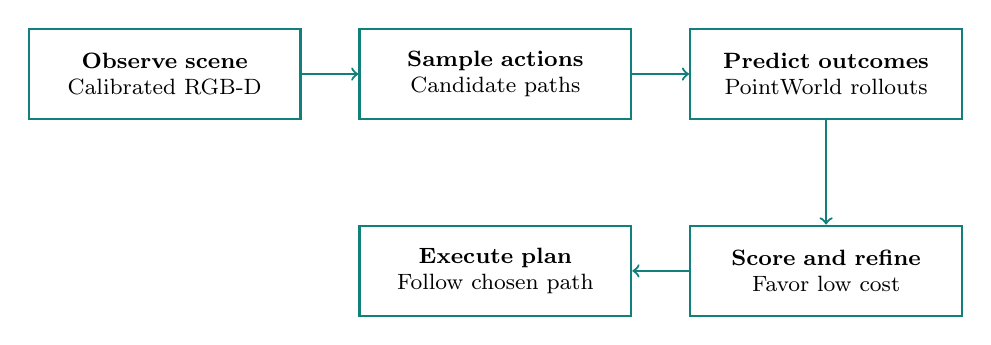
\begin{tikzpicture}[
    every node/.style={font=\footnotesize,align=center},
    stage/.style={draw=pw,thick,text width=3.1cm,minimum height=1.15cm,inner sep=5pt}
  ]
    \node[stage] (obs) at (0,1.5) {\textbf{Observe scene}\\Calibrated RGB-D};
    \uncover<2->{
      \node[stage] (sample) at (4.2,1.5) {\textbf{Sample actions}\\Candidate paths};
      \draw[->,thick,pw] (obs.east)--(sample.west);
    }
    \uncover<3->{
      \node[stage] (pred) at (8.4,1.5) {\textbf{Predict outcomes}\\PointWorld rollouts};
      \draw[->,thick,pw] (sample.east)--(pred.west);
    }
    \uncover<4->{
      \node[stage] (score) at (8.4,-1.0) {\textbf{Score and refine}\\Favor low cost};
      \draw[->,thick,pw] (pred.south)--(score.north);
    }
    \uncover<5->{
      \node[stage] (act) at (4.2,-1.0) {\textbf{Execute plan}\\Follow chosen path};
      \draw[->,thick,pw] (score.west)--(act.east);
    }
  \end{tikzpicture}
  \vfill
 
  \vspace{5pt}
  \credit{\S3.2; real-robot appendix}
\end{frame}


\begin{frame}{MPPI: sampling and optimizing robot trajectories}

  \begin{columns}[c]

    % LEFT: Trajectory visualization
    \column{0.43\textwidth}
      \centering
      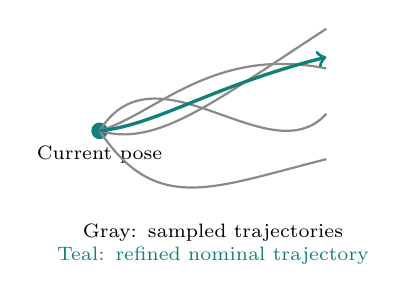
\begin{tikzpicture}[x=0.72cm,y=0.72cm]

        \fill[pw] (0,0) circle (3pt);
        \node[font=\scriptsize,anchor=north]
          at (0,-0.1) {Current pose};

        % Candidate trajectories
        \uncover<1->{
          \draw[mute,thick]
            (0,0)..controls(1,0.3)and(2,1.5)..(4,1.1);
          \draw[mute,thick]
            (0,0)..controls(1,1.6)and(3,-0.8)..(4,0.3);
          \draw[mute,thick]
            (0,0)..controls(1,-1.5)and(2,-1)..(4,-0.5);
          \draw[mute,thick]
            (0,0)..controls(1,-0.3)and(2,0.5)..(4,1.8);
        }

        % Refined nominal trajectory
        \uncover<3->{
          \draw[pw,very thick,->]
            (0,0)..controls(1,0.1)and(2,0.8)..(4,1.3);
        }

        \node[font=\scriptsize,text width=4cm,
              align=center]
          at (2,-2) {
            Gray: sampled trajectories\\
            \textcolor{pw}{Teal: refined nominal trajectory}
          };

      \end{tikzpicture}

    % RIGHT: Technical steps
    \column{0.55\textwidth}

      \footnotesize
      \begin{itemize}
        \setlength{\itemsep}{11pt}

        \item<1-> \textbf{Sample trajectories:}
          Generate $K$ candidate end-effector
          trajectories using time-correlated
          cubic-spline perturbations.

        \item<2-> \textbf{Predict and evaluate:}
          Convert each candidate into robot
          point flows; use PointWorld to predict
          scene motion and compute cost $J^{(\ell)}$.

        \item<3-> \textbf{Update nominal trajectory:}
          Weight candidates by their costs:
      \end{itemize}

      \uncover<3->{
        \vspace{-5pt}
        \[
          \omega_\ell =
          \frac{\exp(-J^{(\ell)}/\beta)}
               {\sum_{\ell'}\exp(-J^{(\ell')}/\beta)}
        \]
      }

  \end{columns}

  \vfill


  \credit{\S3.2; MPPI \citep{williams2017mppi}}
\end{frame}



\begin{frame}{Planning cost: task success + robot motion}

  \vspace{-8pt}
  \small
  \[
    \underset{\mathbf E_{0:T}}{\operatorname{arg\,min}}
    \sum_{k=1}^{T}
    \left[
      \underbrace{c_{\mathrm{task}}(\mathbf s_k)}_{\text{Task cost}}
      +
      \underbrace{c_{\mathrm{ctrl}}(\mathbf E_k)}_{\text{Control cost}}
    \right]
  \]

  \vspace{6pt}

  \begin{itemize}
    \footnotesize
    \setlength{\itemsep}{15pt}

    \item<1-> \textbf{Task cost:} How close does the
      predicted scene get to the desired target?
      \vspace{-4pt}
      \[
        c_{\mathrm{task}}(\mathbf s_k)
        =
        \frac{1}{|\mathcal I_{\mathrm{task}}|}
        \sum_{i\in\mathcal I_{\mathrm{task}}}
        \|\mathbf p_{k,i}-\mathbf g_i\|_2^2
      \]
      {\scriptsize
        $\mathbf p_{k,i}$: predicted point position;
        $\mathbf g_i$: target position;
        $\mathcal I_{\mathrm{task}}$: selected points.
      \par}

    \item<2-> \textbf{Control cost:}
      Evaluates the end-effector trajectory
      $\mathbf E_{0:T}$ by penalizing:
      \begin{itemize}
        \item Excessive travel distance between poses.
        \item Unreachable end-effector poses.
      \end{itemize}

  \end{itemize}

  \vfill


  \credit{Eq.~2, \S3.2}
\end{frame}


%% ==== HANDOFF: Vivian presents S1-3 above, Juntang S4-6 below ====

%% ---- Part B: data and evidence, about 7:45 ----

% 7. Data  1:15  (S4, Fig. 5)
\begin{frame}{Data: re-annotating DROID in 3D}
  \centering
  \paperfig{height=4.0cm}{figs/fig5a_annotation.pdf}{Fig.~5, top}
  \vfill
  \begin{notes}[0.86\linewidth]
    \item DROID \src{khazatsky2024droid}: real teleoperation, but its depth and camera
      poses are off. Three fixes: depth from FoundationStereo \src{wen2025foundationstereo}, poses
      from VGGT \src{wang2025vggt} refined against the robot mesh, CoTracker3
      \src{karaev2025cotracker3} tracks lifted to 3D
    \item \pw{Over 60\% of DROID survives, about 200 hours}. With BEHAVIOR-1K simulation
      \src{li2024behavior}, the total is about 2M trajectories, 500 hours
  \end{notes}
  \vfill
\end{frame}

% 8. How it is scored  0:45  (S4 evaluation protocol, Fig. 6 top two rows)
\begin{frame}{How it is scored}
  \centering
  \paperfig{width=0.92\linewidth, trim=16 485 0 0, clip}{figs/fig6_rollouts.pdf}{Fig.~6, top two rows}
  \vfill
  \begin{notes}[0.92\linewidth]
    \item \textbf{$\ell_2$ mover}: mean distance, in metres, between predicted and true
      positions of the points that move, over the 1\,s horizon
    \item On DROID, points count only where a separate model, trained on the test split, is
      confident (\S4: the top 80\%)
    \item \pw{0.001 is one millimetre. Read every difference that follows in mm}
  \end{notes}
  \vfill
\end{frame}

% 9. Roadmap  1:00  (Fig. 7, S5.1)
\begin{frame}{Recipe: what each change bought}
  \begin{columns}[c]
    \column{0.40\textwidth}
      \centering
      \paperfig{height=6.0cm}{figs/fig7_roadmap.pdf}{Fig.~7}
    \column{0.58\textwidth}
      \footnotesize
      \begin{itemize}\setlength{\itemsep}{5pt}
        \item Swapping the graph network (GBND) for PTv3 is the biggest single step:
          0.0386 to 0.0348
        \item The loss and DINO image features add 1.7\,mm; scaling PTv3 from 50M to 1B
          parameters adds 1.9\,mm
        \item \pw{0.0386 to 0.0312 overall: 7.4\,mm, or 19\% less error on moving points}
      \end{itemize}
      \vspace{4pt}
      {\scriptsize\color{mute} Each bar adds one change to the bar above it. Hatched bars
        were tried and not kept.\par}
  \end{columns}
\end{frame}

% 10. Scaling  0:45  (Fig. 9, S5.2 scaling paragraph; Tab. 1 for memory and latency)
\begin{frame}{Scaling}
  \begin{columns}[c]
    \column{0.42\textwidth}
      \centering
      \paperfig{height=4.7cm}{figs/fig9_scaling.pdf}{Fig.~9}
    \column{0.56\textwidth}
      \footnotesize
      \begin{itemize}\setlength{\itemsep}{5pt}
        \item Error falls roughly log-linearly with data, from 5\% to 100\% of DROID, and
          with model size, from 50M to 1B parameters
        \item PTv3 makes the model axis affordable: 957 times GBND's parameters for 4.3
          times the memory, about 0.12\,s per pass at 1B (Tab.~1)
        \item \pw{Predictable gains from more data and capacity, as in language and vision}
      \end{itemize}
      \vspace{4pt}
      {\scriptsize\color{mute} One axis at a time, on DROID. All nine backbones in the
        backup.\par}
  \end{columns}
\end{frame}

% 11. Why gripper points  0:45  (Fig. 11, S5.2) -- first to cut if running long
\begin{frame}{Why gripper points?}
  \begin{columns}[c]
    \column{0.44\textwidth}
      \centering
      \paperfig{height=4.4cm}{figs/fig11_action.pdf}{Fig.~11}
    \column{0.54\textwidth}
      \footnotesize
      \begin{itemize}\setlength{\itemsep}{5pt}
        \item Robot as points on its grippers only, against points on the whole body (two
          densities), end-effector pose, or joint positions
        \item Lowest error on both real (DROID) and simulated (B1K) data. On real data,
          whole-body points do worse than a plain pose; the authors' reading: too many robot
          points drown the few moving scene points
        \item \pw{Gripper points keep the contact geometry and stay the same format for
          both robots}
      \end{itemize}
      \vspace{4pt}
      {\scriptsize\color{mute} All variants are trained on DROID and B1K together. The
        paper does not say what the markers above the bars are.\par}
  \end{columns}
\end{frame}

% 12. Transfer to a new lab  1:00  (Tab. 2 held-out columns, S5.3; finetuning = 1/20
%     of the iterations)
\begin{frame}{Does it transfer to a new lab?}
  \centering\small
  \setlength{\tabcolsep}{9pt}
  \begin{tabular}{@{}lcccc@{}}
    \toprule
    pretrained on & DROID & BEHAVIOR-1K & \pw{both} & specialist (H only) \\
    \midrule
    zero-shot & 0.0305 & 0.0531 & \pw{0.0300} & 0.0293 \\
    finetuned & \textbf{0.0271} & 0.0299 & \pw{\textbf{0.0272}} & 0.0293 \\
    \bottomrule
  \end{tabular}
  \credit{Tab.~2, held-out columns, $\ell_2$ mover; in- and cross-domain columns in the
    backup}
  \vfill
  \begin{notes}[0.9\linewidth]
    \item H: one DROID lab held out of pretraining. The specialist trains on that lab alone
    \item Zero-shot, real-plus-sim pretraining comes within 0.7\,mm of the specialist.
      \pw{Finetuned with 1/20 of the training steps, it beats the specialist by 2.1\,mm}
    \item Simulation alone does not transfer zero-shot, but finetuning brings it close to
      the specialist
  \end{notes}
  \vfill
\end{frame}

% 13. Real robot  1:15  (Fig. 8, S5.4, App. real-robot details)
\begin{frame}{Results: real robot, zero-shot}
  \centering
  \includegraphics[height=2.7cm]{figs/fig8b_tasks.pdf}\\[1pt]
  \includegraphics[width=0.86\linewidth]{figs/fig8a_success.pdf}
  \credit{Fig.~8}
  \vspace{2pt}
  \begin{notes}[0.9\linewidth]
    \item 8 tasks $\times$ 10 trials, one camera, a gripper never seen in training, no demos
      or finetuning: \pw{56\% overall (45 of 80)}
    \item Each plan runs without replanning; the deformable and tool tasks start with the object
      grasped. Videos: \href{https://point-world.github.io}{point-world.github.io}
  \end{notes}
\end{frame}

% 14. Limitations  0:30  (App. "Extended Discussions on Limitations")
\begin{frame}{Limitations}
  \vfill
  \begin{columns}
    \column{0.86\textwidth}
      {\small\bfseries Stated by the authors} {\scriptsize\color{mute}(Appendix)}
      \vspace{4pt}
      \begin{itemize}\setlength{\itemsep}{6pt}
        \item One still frame in, so the scene must start at rest: no velocities
        \item Task costs are drawn by hand: object masks and target points
        \item The robot is assumed rigid and to follow its planned path exactly
      \end{itemize}
  \end{columns}
  \vfill
\end{frame}

% 15. Takeaway  0:30
\begin{frame}{Takeaway}
  \vfill
  \begin{columns}
    \column{0.88\textwidth}
      \begin{itemize}\setlength{\itemsep}{10pt}
        \item \pw{One 3D world model for more than one robot: scene and action as moving
          points, trained on 2M real and simulated trajectories}
        \item Each piece of the recipe lowers the error, and more data and parameters keep
          helping at a predictable rate
        \item From a single image it plans real pushing, cloth, hinge and tool tasks
          zero-shot; code, data and checkpoints are public
      \end{itemize}
  \end{columns}
  \vfill
\end{frame}

% 16. Discussion  -- the 15 minutes end here; call on the roles in the agreed order.
%     Each question hands a thread to a role (reviewer, red team, researcher).
\begin{frame}{Discussion}
  \begin{itemize}\setlength{\itemsep}{6pt}
    \item The robot results report no baseline and never replan. What comparison would
      show that 56\% is good?
    \item On real data a plain end-effector pose comes close to gripper points. Is the
      point action essential, or mainly a way to mix robots?
    \item The model sees one frozen frame, and moving points are still off by about
      3\,cm. Which tasks does that rule out?
  \end{itemize}
\end{frame}

%% ---- backup ----
\appendix

% Our critique, kept out of the main talk (presenter = first author). Sources: S4, S5.2,
% S5.3, S5.4, App. DROID evaluation protocol, App. real-robot details.
\begin{frame}{Backup: our reading}
  \footnotesize
  \begin{itemize}\setlength{\itemsep}{5pt}
    \item \textbf{Robot}: 8 tasks $\times$ 10 trials, no baseline success rate, no
      replanning, deformable and tool tasks start pre-grasped. 56\% cannot yet be ranked
      against a policy or another model
    \item \textbf{Metric}: real-data gaps are a few mm, scored on points an expert model
      trusts. \S4 says it keeps the top 80\%; the appendix thresholds ``at the 0.8
      quantile'' and drops the points below, which reads as the top 20\%
    \item \textbf{Transfer}: zero-shot on a held-out lab is 0.7\,mm behind the specialist;
      the clear wins need finetuning
    \item \textbf{Small inconsistencies}: GBND is 0.0390 in Tab.~1 and 0.0386 in Fig.~7.
      Fig.~11's legend gives whole-body variants of 500 and 3000 points; \S5.2 gives ``the
      same number of points'' and 2000
  \end{itemize}
\end{frame}

% Eq. 1 and the movement weight, S3.1
\begin{frame}{Backup: training objective}
  \small
  \[
    \tfrac12 \sum_{k,i}^{H, N_S}
    \underbrace{w_{k,i}}_{\text{movement}}
    \Big( \underbrace{\rho_\delta\big(\hat P_{t+k,i} - P_{t+k,i}\big)}_{\text{Huber on 3D residual}}
    \underbrace{e^{-s_{k,i}}}_{\text{uncertainty weight}}
    + \underbrace{s_{k,i}}_{\text{regularizer}} \Big)
    \tag{1}
  \]
  \[
    m_{k,i} = \sigma\big(\kappa(\delta_{k,i} - \tau)\big), \qquad
    w_{k,i} = m_{k,i} \Big/ \textstyle\sum_{k,i} m_{k,i}
  \]
  \credit{\S3.1}
  \vfill
  \begin{notes}
    \item $\delta_{k,i}$: length of point $i$'s true displacement at step $k$; $\tau$ a
      threshold, $\kappa$ a temperature
    \item Points the 2D tracker marks as occluded get no loss at all
    \item Aleatoric uncertainty, the same device VGGT uses \src{wang2025vggt}: the model may
      say ``unsure'', at the price of the $s$ term
  \end{notes}
\end{frame}

% App. real-robot details
\begin{frame}{Backup: planning and robot protocol}
  \footnotesize
  \begin{columns}[t]
    \column{0.48\textwidth}
      {\small\bfseries Planner}
      \begin{itemize}\setlength{\itemsep}{2pt}
        \item MPPI around a zero nominal, cubic-spline noise (4 knots), $\sigma$ from 0.05
          to 0.50
        \item 256 samples, temperature $\beta = 0.05$, EMA 0.9, 20 iterations
        \item 30 steps ahead, in 3 chunked passes; no replanning in this work
      \end{itemize}
    \column{0.48\textwidth}
      {\small\bfseries Robot}
      \begin{itemize}\setlength{\itemsep}{2pt}
        \item 7-DoF Franka on a wheeled base, 3D-printed fin-ray gripper (training saw
          Robotiq and Galaxea R1 Pro grippers)
        \item One RealSense D435; depth from its stereo IR pair via FoundationStereo
        \item Masks from SAM~2 \src{ravi2024sam2}, targets placed in a GUI; failures include
          plans judged unsafe to run
      \end{itemize}
  \end{columns}
  \vspace{4pt}\credit{Appendix, real-robot experiment details}
\end{frame}

\begin{frame}{Backup: all backbones}
  \centering\small
  \setlength{\tabcolsep}{5pt}
  \begin{tabular}{@{}lrrrrrr@{}}
    \toprule
    & params & memory & FLOPs & latency (ms) & $\ell_2$ mover & $\ell_2$ static \\
    \midrule
    GBND \src{ai2025review} & 1.00$\times$ & 1.00$\times$ & 1.00$\times$ & 13.46 & 0.0390 & 0.0066 \\
    PointNet & 1.03$\times$ & 0.34$\times$ & 0.04$\times$ & 5.93 & 0.0369 & 0.0084 \\
    PointNet++ & 1.07$\times$ & 0.67$\times$ & 0.06$\times$ & 327.08 & 0.0368 & 0.0073 \\
    SparseConv & 33.31$\times$ & 7.18$\times$ & 1.32$\times$ & 17.70 & 0.0396 & 0.0076 \\
    Transformer & 41.06$\times$ & 0.31$\times$ & 3.38$\times$ & 30.43 & 0.0339 & 0.0071 \\
    \pw{PTv3-50M} & 49.14$\times$ & 0.30$\times$ & 0.34$\times$ & 59.60 & 0.0331 & 0.0067 \\
    \pw{PTv3-132M} & 127.22$\times$ & 0.69$\times$ & 1.04$\times$ & 69.60 & 0.0324 & 0.0061 \\
    \pw{PTv3-411M} & 398.67$\times$ & 1.89$\times$ & 1.90$\times$ & 102.47 & 0.0315 & 0.0059 \\
    \pw{PTv3-1B} & 957.71$\times$ & 4.30$\times$ & 3.57$\times$ & 123.65 & \textbf{0.0312}
      & \textbf{0.0056} \\
    \bottomrule
  \end{tabular}
  \credit{Tab.~1, relative to GBND}
  \vspace{4pt}
  \begin{notes}[0.86\linewidth]
    \item GBND keeps a feature for every point and passes messages only locally, so memory
      grows fast and far-away effects get lost
  \end{notes}
\end{frame}

\begin{frame}{Backup: generalization, all columns}
  \centering\scriptsize
  \setlength{\tabcolsep}{5pt}
  \begin{tabular}{@{}ll*{7}{c}c@{}}
    \toprule
    & & D$\to$D & B$\to$B & D$\to$B & B$\to$D & D$\to$H & B$\to$H & D+B$\to$H & specialist \\
    \midrule
    zero-shot & mover & 0.0315 & 0.0087 & 0.1460 & 0.0558 & 0.0305 & 0.0531 & 0.0300 & 0.0293 \\
      & static & 0.0059 & 0.0010 & 0.0050 & 0.0058 & 0.0049 & 0.0057 & 0.0063 & 0.0043 \\
    \midrule
    finetuned & mover & -- & -- & 0.0107 & 0.0378 & 0.0271 & 0.0299 & 0.0272 & 0.0293 \\
      & static & -- & -- & 0.0003 & 0.0086 & 0.0040 & 0.0046 & 0.0040 & 0.0043 \\
    \bottomrule
  \end{tabular}
  \credit{Tab.~2: D = DROID, B = BEHAVIOR-1K, H = held-out lab}
  \vspace{6pt}
  \paperfig{height=2.4cm}{figs/fig10_heldout.pdf}{Fig.~10}\par\vspace{6pt}
  {\tiny\color{mute} H is the CLVR lab within DROID, split 90/10; finetuned models see only
    the 90\%. Zero-shot across sim and real fails both ways (0.1460, 0.0558).\par}
\end{frame}

% Fig. 12, S5.2
\begin{frame}{Backup: predict 1\,s at once}
  \begin{columns}[c]
    \column{0.52\textwidth}
      \centering
      \paperfig{width=\linewidth}{figs/fig12_chunk.pdf}{Fig.~12}
    \column{0.46\textwidth}
      \footnotesize
      \begin{itemize}\setlength{\itemsep}{5pt}
        \item Predicting all 10 steps together drifts least, in one pass instead of 2 to 10
        \item The same model fed its own outputs one step at a time drifts most
        \item The planner chains three such chunks to look 3\,s ahead
      \end{itemize}
  \end{columns}
\end{frame}

% Fig. 13, S5.2
\begin{frame}{Backup: cameras}
  \centering
  \paperfig{height=4.6cm}{figs/fig13_cameras.pdf}{Fig.~13}
  \vfill
  \begin{notes}[0.8\linewidth]
    \item More cameras in training help at every test setting
    \item Training on a random draw of up to three cameras is the most robust
  \end{notes}
\end{frame}

\begin{frame}{Backup: annotation quality}
  \centering
  \paperfig{width=0.95\linewidth}{figs/fig5b_cdf.pdf}{Fig.~5, bottom}
  \vfill
  \begin{notes}
    \item Left: depth reprojection error on the robot's own surface. Right: point cloud
      agreement between two cameras within 5 and 20\,mm
    \item Off-the-shelf models alone (FoundationStereo, VGGT) are not enough; the robot-mesh
      refinement is what lifts the curves
    \item Extrinsics land a median 1.8\,cm and 1.9$^\circ$ from a proxy truth: the best 1\% of
      scenes under DROID's own calibration
  \end{notes}
\end{frame}

% No allowframebreaks: with it, multicols emits a blank page and clips the last entry.
\begin{frame}[t]{References}
  \vspace{-1.2em}
  \nocite{huang2026pointworld}
  {\tiny\linespread{0.84}\selectfont
  \setlength{\bibsep}{0.2pt plus 0.2pt}
  \setlength{\columnsep}{1em}
  \begin{multicols}{2}\bibliography{refs}\end{multicols}}
\end{frame}

\end{document}
